\documentclass{HW} % requires HW.cls in the same directory

\HWauthor{Bobby Zhong}{bobbyzyz@sas.upenn.edu}
\HWno{1}
\HWcourse{STAT 5200}

\usepackage[T1]{fontenc}
\usepackage{lmodern}
\usepackage{amsmath}
\usepackage{amssymb}
\usepackage{booktabs}
\usepackage{graphicx}
\usepackage{float}
\usepackage{xcolor}
\usepackage{listings}
\usepackage{hyperref}
\hypersetup{colorlinks=true, linkcolor=blue!50!black, urlcolor=blue!50!black}

\lstset{
  language=R, basicstyle=\ttfamily\footnotesize,
  keywordstyle=\color{blue!60!black}\bfseries, commentstyle=\color{green!40!black}\itshape,
  stringstyle=\color{red!60!black}, frame=single, rulecolor=\color{gray!60},
  backgroundcolor=\color{gray!5}, breaklines=true, showstringspaces=false,
  columns=fullflexible, keepspaces=true
}
\lstdefinestyle{routput}{
  language={}, basicstyle=\ttfamily\footnotesize, frame=single, rulecolor=\color{gray!60},
  backgroundcolor=\color{white}, keywordstyle=\ttfamily, commentstyle=\ttfamily, stringstyle=\ttfamily
}

\newcommand{\E}{\mathbb{E}}
\newcommand{\Var}{\operatorname{Var}}

\begin{document}
\maketitle

%%%%%%%%%%%%%%%%%%%%%%%%%%%%%%%%%%%%%%%%%%%%%%%%%%%%%%%%%%%%%%%%%%%%%%%%%%%%%%
\section*{Question 1}
%%%%%%%%%%%%%%%%%%%%%%%%%%%%%%%%%%%%%%%%%%%%%%%%%%%%%%%%%%%%%%%%%%%%%%%%%%%%%%

\subsection*{1.2 Matrix computations}

\noindent\textbf{(a)}

\begin{lstlisting}
A <- matrix(c(5, 2, 2, 1), nrow = 2, byrow = TRUE)
B <- matrix(c(5, 2, 2, 5), nrow = 2, byrow = TRUE)
\end{lstlisting}

\medskip
\noindent\textbf{(b)}

\begin{lstlisting}
C <- solve(A) %*% B   # C = A^{-1} B
\end{lstlisting}
The determinant of $A$ is $\det A = 5 \cdot 1 - 2 \cdot 2 = 1$, so that
\[ A^{-1} = \begin{pmatrix} 1 & -2 \\ -2 & 5 \end{pmatrix} \qquad \text{and} \qquad C = A^{-1}B = \begin{pmatrix} 1 & -2 \\ -2 & 5 \end{pmatrix} \begin{pmatrix} 5 & 2 \\ 2 & 5 \end{pmatrix} = \begin{pmatrix} 1 & -8 \\ 0 & 21 \end{pmatrix}. \]
The output of R agrees with this calculation.

\medskip
\noindent\textbf{(c)}

\begin{lstlisting}
print(t(C))           # transpose of C
\end{lstlisting}
\begin{lstlisting}[style=routput]
     [,1] [,2]
[1,]    1    0
[2,]   -8   21
\end{lstlisting}
Hence
\[ C' = \begin{pmatrix} 1 & 0 \\ -8 & 21 \end{pmatrix}. \]

\medskip
\noindent\textbf{(d)}

\begin{lstlisting}
print(A %*% B)        # matrix product
print(A * B)          # element-wise product
\end{lstlisting}
\begin{lstlisting}[style=routput]
     [,1] [,2]
[1,]   29   20
[2,]   12    9
     [,1] [,2]
[1,]   25    4
[2,]    4    5
\end{lstlisting}
The operator \texttt{\%*\%} performs matrix multiplication. The $(i,j)$ entry of \texttt{A \%*\% B} is
\[ (AB)_{ij} = \sum_{k} A_{ik} B_{kj}, \]
which requires the number of columns of $A$ to equal the number of rows of $B$; in general, $AB \neq BA$. The operator \texttt{*} performs element-wise multiplication. The $(i,j)$ entry of \texttt{A * B} is
\[ (A * B)_{ij} = A_{ij} B_{ij}, \]
which requires $A$ and $B$ to have the same dimensions; this product is commutative.

\subsection*{1.3 Sum of matrices with a \texttt{for} loop}
\begin{lstlisting}
X <- matrix(0, 2, 2)
for (k in 1:100) {
  D_k <- matrix(c(k, k + 1, k^2, k / 2), nrow = 2, byrow = TRUE)
  X <- X + D_k
}
print(X)
\end{lstlisting}
\begin{lstlisting}[style=routput]
       [,1] [,2]
[1,]   5050 5150
[2,] 338350 2525
\end{lstlisting}
Therefore,
\[ X = \sum_{k=1}^{100} D_k = \begin{pmatrix} 5050 & 5150 \\ 338350 & 2525 \end{pmatrix}, \]
which agrees with the closed-form sums $\sum_{k=1}^{100} k = 5050$, $\sum_{k=1}^{100} (k+1) = 5150$, $\sum_{k=1}^{100} k^2 = 338{,}350$, and $\sum_{k=1}^{100} k/2 = 2525$.

%%%%%%%%%%%%%%%%%%%%%%%%%%%%%%%%%%%%%%%%%%%%%%%%%%%%%%%%%%%%%%%%%%%%%%%%%%%%%%
\section*{Question 2}
%%%%%%%%%%%%%%%%%%%%%%%%%%%%%%%%%%%%%%%%%%%%%%%%%%%%%%%%%%%%%%%%%%%%%%%%%%%%%%

\subsection*{2.1 Simulation}
The population model is
\[ y = \beta_0 + \beta_1 x + \beta_2 x^2 + \varepsilon, \qquad \beta_0 = 1,\quad \beta_1 = 1,\quad \beta_2 = 0.2,\quad x \sim N(1,4), \]
where the error term is now $\varepsilon = v - 20$ with $v \sim \chi^2(20)$. Because $\E[v] = 20$ and $\Var(v) = 40$, the new error term has mean zero and variance $40$, and its distribution is right-skewed. Under the original model, the error term follows a symmetric distribution with variance $\Var(t_{10}) = 1.25$. Since the mean of the error term is unchanged, the population object of interest is also unchanged:
\[ \theta_0 = \E[y] = \beta_0 + \beta_1 \E[x] + \beta_2 \E[x^2] + \E[\varepsilon] = 1 + 1 + 0.2 \cdot 5 + 0 = 3. \]
For the sample mean $\hat\theta$ computed from a random sample of size $N$,
\[ \begin{gathered} \Var(\hat\theta) = \frac{\Var(y)}{N}, \qquad \Var(\sqrt{N}\hat\theta) = \Var(y), \\ \Var(y) = \Var(x + 0.2x^2) + \Var(\varepsilon) = 9.12 + \Var(\varepsilon), \end{gathered} \]
so that $\Var(y) = 10.37$ under the original model and $\Var(y) = 49.12$ under the new model.

For each model and each $N \in \{20, 100, 500\}$, $M = 1000$ data sets are generated, the sample mean of $y$ is computed for each data set, and the variances of $\hat\theta$ and of $\sqrt{N}\hat\theta$ across the $M$ replications are recorded.

\begin{lstlisting}
set.seed(1)
M <- 1000
z500 <- list()   # sqrt(N) * theta_hat for N = 500, one vector per model
for (err in c("t10", "chisq20")) {
  for (N in c(20, 100, 500)) {
    theta_hat <- numeric(M)
    for (m in 1:M) {
      x <- rnorm(N, mean = 1, sd = 2)
      e <- if (err == "t10") rt(N, df = 10) else rchisq(N, df = 20) - 20
      y <- 1 + x + 0.2 * x^2 + e
      theta_hat[m] <- mean(y)
    }
    cat(sprintf("%-7s N = %3d  Var(theta_hat) = %.5f  Var(sqrt(N) theta_hat) = %.3f\n",
                err, N, var(theta_hat), N * var(theta_hat)))
    if (N == 500) z500[[err]] <- sqrt(N) * theta_hat
  }
}
print(rbind(mean = sapply(z500, mean), sd = sapply(z500, sd)))

png("fig_q2_hist.png", width = 1800, height = 800, res = 200)
par(mfrow = c(1, 2))
xlim <- range(unlist(z500))
xlab <- "sqrt(N) * theta_hat, N = 500"
hist(z500$t10, breaks = 40, xlim = xlim, xlab = xlab,
     main = "Original model: e ~ t(10)")
hist(z500$chisq20, breaks = 40, xlim = xlim, xlab = xlab,
     main = "New model: e = v - 20, v ~ chi-squared(20)")
dev.off()
\end{lstlisting}
\begin{lstlisting}[style=routput]
t10     N =  20  Var(theta_hat) = 0.53733  Var(sqrt(N) theta_hat) = 10.747
t10     N = 100  Var(theta_hat) = 0.10308  Var(sqrt(N) theta_hat) = 10.308
t10     N = 500  Var(theta_hat) = 0.02030  Var(sqrt(N) theta_hat) = 10.150
chisq20 N =  20  Var(theta_hat) = 2.63504  Var(sqrt(N) theta_hat) = 52.701
chisq20 N = 100  Var(theta_hat) = 0.51756  Var(sqrt(N) theta_hat) = 51.756
chisq20 N = 500  Var(theta_hat) = 0.09791  Var(sqrt(N) theta_hat) = 48.953
           t10  chisq20
mean 66.919592 67.21585
sd    3.185886  6.99665
\end{lstlisting}

\subsection*{2.2 Do we arrive at the same conclusion?}
Yes.
\begin{itemize}
\item The sampling uncertainty of $\hat\theta$ decreases as $N$ increases, and it does so by approximately a factor of five whenever $N$ is multiplied by five. Under the new model, $\Var(\hat\theta)$ falls from $2.64$ to $0.52$ and then to $0.098$, with ratios of $5.1$ and $5.3$; under the original model, it falls from $0.54$ to $0.10$ and then to $0.020$.
\item The variance of $\sqrt{N}\hat\theta$ does not decrease with $N$. Under the new model it remains between $49$ and $53$, close to the theoretical value $\Var(y) = 49.12$, and under the original model it remains close to $10$, in line with $\Var(y) = 10.37$.
\item The two models differ only in the level of the sampling uncertainty. Every variance is roughly five times larger under the new model because $\Var(\varepsilon)$ increases from $1.25$ to $40$, whereas the rate at which the uncertainty vanishes, namely $1/N$, depends only on $\Var(y)$ and not on the shape of the error distribution.
\end{itemize}

\subsection*{2.3 Histogram of $\sqrt{N}\hat\theta$ for $N = 500$}
\begin{figure}[H]
\centering
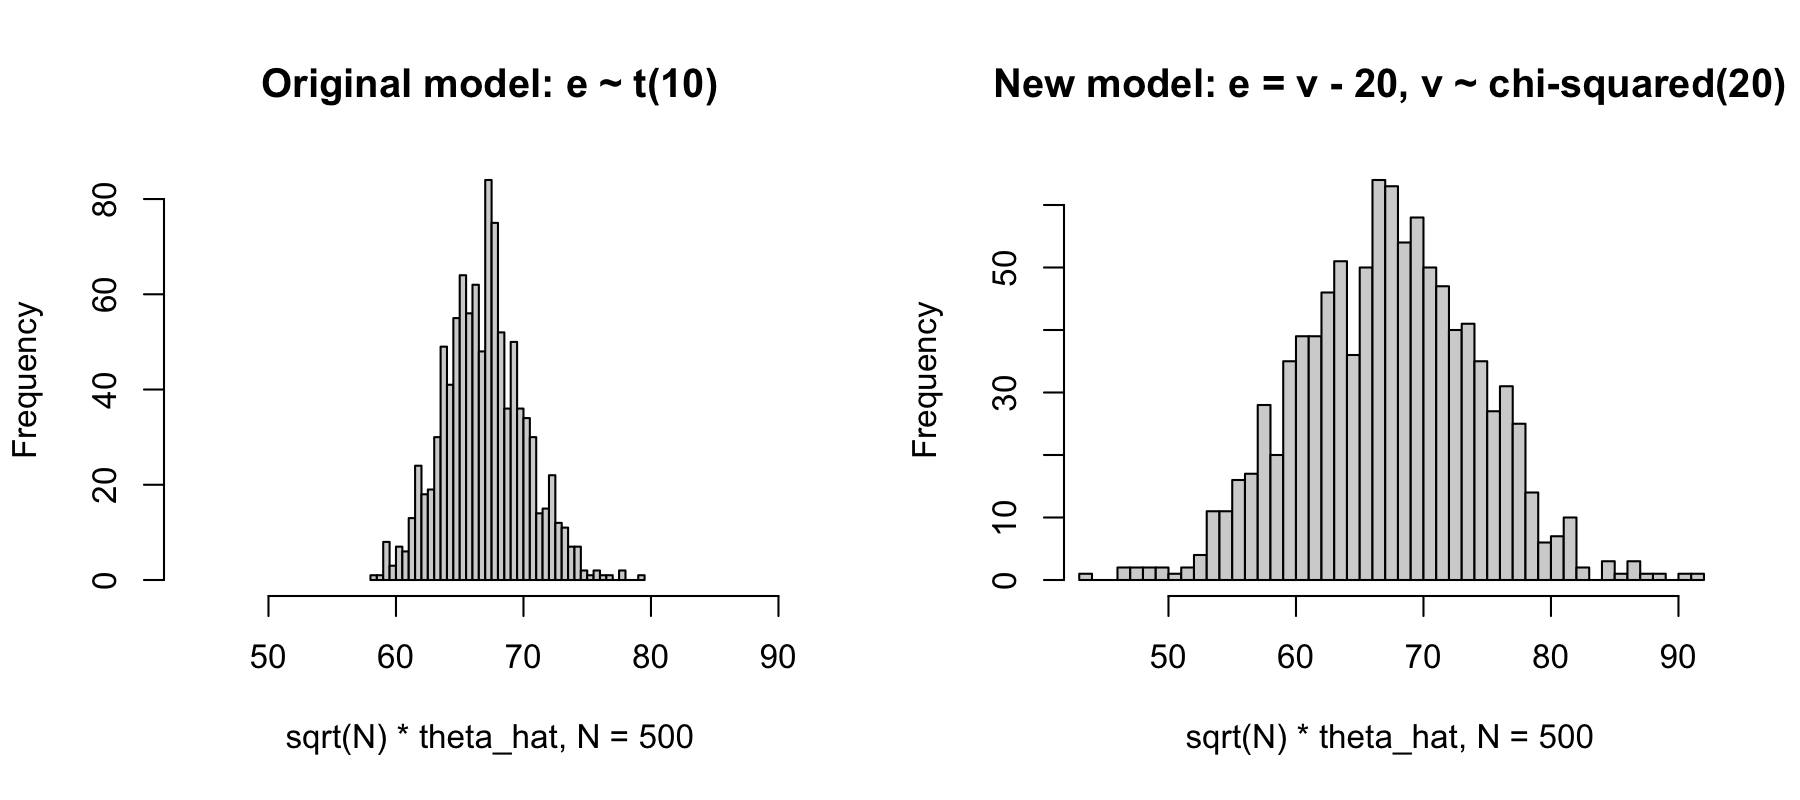
\includegraphics[width=\textwidth]{fig_q2_hist.png}
\caption{Histograms of $\sqrt{N}\hat\theta$ with $N = 500$ over $M = 1000$ replications under the original model (left) and under the new model (right). Both panels use the same horizontal axis.}
\end{figure}
The two histograms are similar in shape but differ in scale. Both are unimodal, approximately symmetric, and bell-shaped, and both are centered at $\sqrt{500} \cdot 3 \approx 67.1$; the sample means are $66.9$ and $67.2$. Although the $\chi^2$ error term is right-skewed, the skewness is averaged out over $N = 500$ observations, as the central limit theorem predicts. The histogram for the new model is, however, approximately $2.2$ times wider, with a standard deviation of $7.0$ rather than $3.2$, which matches the ratio $\sqrt{49.12/10.37} \approx 2.2$ implied by the larger value of $\Var(y)$.

%%%%%%%%%%%%%%%%%%%%%%%%%%%%%%%%%%%%%%%%%%%%%%%%%%%%%%%%%%%%%%%%%%%%%%%%%%%%%%
\section*{Question 3}
%%%%%%%%%%%%%%%%%%%%%%%%%%%%%%%%%%%%%%%%%%%%%%%%%%%%%%%%%%%%%%%%%%%%%%%%%%%%%%

\subsection*{3.1 Field}
The field of interest is the economics of information systems, which studies how changes in the availability and use of information, driven by information technology, affect consumer behavior, competition, and market structure.

\subsection*{3.2 Journals}
\begin{enumerate}
\item MS: \emph{Management Science}
\item ISR: \emph{Information Systems Research}
\item MISQ: \emph{MIS Quarterly} (\emph{Management Information Systems Quarterly})
\item JMIS: \emph{Journal of Management Information Systems}
\item POM: \emph{Production and Operations Management}
\end{enumerate}

\subsection*{3.3 The paper}
The selected paper is Wu, Lou, and Hitt (2025), ``Innovation Strategy After IPO: How AI Analytics Spurs Innovation After IPO,'' published in \emph{Management Science}. The paper contains the word ``econometric,'' as the authors rely on the textbook \emph{Econometric Analysis of Cross Section and Panel Data} by Wooldridge for their selection correction and apply panel data econometric methods throughout the empirical analysis. These methods are applied to a panel of 1{,}471 firms observed from 1988 to 2013, and the estimation results are reported in the tables of the paper.

\subsection*{3.4 Citation}
Wu, L., Lou, B., \& Hitt, L.\ M.\ (2025). Innovation strategy after IPO: How AI analytics spurs innovation after IPO. \emph{Management Science}, \emph{71}(3), 2360--2389. \url{https://doi.org/10.1287/mnsc.2022.01559}

\subsection*{3.5 Main research question}
The innovation quality of firms is known to decline after an initial public offering (IPO). The literature attributes this decline to short-term financial pressure, to disclosure requirements, and to weaker managerial incentives, and the available remedies, such as leveraged buyouts, acquisitions, or remaining private, are costly. The paper asks whether the acquisition of AI analytics capability, measured by the number of employees with data analytics and machine learning skills, mitigates the post-IPO decline in innovation quality, and through which channels any such effect operates. The authors hypothesize that AI analytics is most useful for innovations that recombine existing technologies rather than for radically new inventions. Using patent-based measures of innovation quality, they find that firms that build AI analytics capability after going public experience a significantly smaller decline in patent originality and in new-combination patents but no improvement in radically new inventions. They also find that the effect operates through the short-termism and disclosure channels but not through the managerial incentive channel, and that firms increase their hiring of AI talent in the years following the IPO.

\subsection*{3.6 Econometric methods}
\begin{itemize}
\item A panel data regression with firm and year fixed effects in a difference-in-differences design, which compares public and private firms before and after the IPO and interacts AI analytics with post-IPO status; this is the main specification.
\item Event-study regressions with leads and lags around the IPO year.
\item Propensity score matching and coarsened exact matching, together with a Rosenbaum bounds sensitivity analysis.
\item The Heckman two-stage selection model, with a probit first stage and an inverse Mills ratio correction.
\item Instrumental variables estimation by two-stage least squares, also combined with the Heckman correction and with the matched sample.
\end{itemize}

\subsection*{3.7 Standard errors}
Yes. Every regression table reports the standard error of each coefficient in parentheses below the estimate. The table notes state that robust standard errors are clustered by firm, and significance levels are indicated by stars for $p < 0.01$, $p < 0.05$, and $p < 0.1$. For example, in Table 4 the coefficient on the interaction between $\ln(\text{Analytics})$ and the post-IPO indicator in the regression for patent originality is $0.00982$, with a standard error of $0.00191$. The Heckman tables also report bootstrapped standard errors, and Figure 1 displays confidence intervals around the event-study estimates.

\subsection*{3.8 What is a standard error?}
The standard error of an estimator is the standard deviation of its sampling distribution. It measures how much the estimate would vary across repeated random samples of the same size drawn from the same population. Question 2 is precisely this thought experiment. For the sample mean,
\[ \mathrm{SE}(\hat\theta) = \sqrt{\frac{\Var(y)}{N}}, \]
and the standard deviation of the $1000$ simulated sample means is a Monte Carlo estimate of this quantity. In practice only one sample is observed, so the standard error itself must be estimated from the data, for example by $s/\sqrt{N}$ for a sample mean, or by the square root of the corresponding diagonal element of the estimated covariance matrix of $\hat\beta$ for a regression coefficient. Standard errors that are clustered by firm allow the regression errors to be correlated over time within the same firm. The ratio of an estimate to its standard error is the $t$ statistic from which the $p$ values and significance stars in the tables of the paper are obtained, and the interval $\hat\beta \pm 1.96\,\mathrm{SE}$ is an approximate 95 percent confidence interval.

\end{document}
